\documentclass[a4paper]{amsart}

\newif\iflmcs\lmcsfalse % <--------------- TOGGLE THIS FOR FINAL VERSION OF LMCS
                        %                  Trash .aux file after toggling
\usepackage{stmaryrd}
\usepackage{graphicx}
\usepackage[lutzsyntax]{virginialake}\vlsmallbrackets\aftrianglefalse
\iflmcs\def\url #1#2{\relax}\else\usepackage{hyperref}\fi

%--------- Theorem etc
\newtheorem{thm}{Theorem}[section]
\newtheorem{cor}[thm]{Corollary}
\newtheorem{lem}[thm]{Lemma}
\newtheorem{pro}[thm]{Proposition}

\theoremstyle{remark}
\newtheorem{rem}[thm]{Remark}

\theoremstyle{definition}
\newtheorem{defi}[thm]{Definition}
%---------

%-------------------------------------------------------- REMOVE WHEN PAPER DONE
\newcommand{\Ale}[1]{{\color{NavyBlue}\noindent {\bf A:} #1}}
\newcommand{\Tom}[1]{{\color{PineGreen}\noindent {\bf T:} #1}}
\newcount\todocount\todocount=0
\newcommand{\TODO}[1]{\global\advance\todocount by1%
            {\color{Red}\noindent{\bf\the\todocount\ TODO:} #1}}\vlupdate{\TODO}
%\renewcommand{\Ale}[1]{\relax}  % Comment/uncomment these three lines
%\renewcommand{\Tom}[1]{\relax}  % in order to display/hide inline comments
%\renewcommand{\TODO}[1]{\relax} %
%-------------------------------------------------------- REMOVE WHEN PAPER DONE

\begin{document}

\title[Normalisation Control in Deep Inference   via Atomic Flows II]
      {Normalisation Control in Deep Inference\\ via Atomic Flows II}

\author{Alessio Guglielmi}
\address{University of Bath, Bath BA2 7AY, UK}

\author{Tom Gundersen}
\iflmcs\address{University of Bath, Bath BA2 7AY, UK}\fi

\thanks{This work was in part funded by an Overseas Research Scholarship and a Research Studentship, both from the University of Bath, and by the British Council Alliance Programme.}

\keywords{Normalisation, deep inference, cut elimination, atomic flows}

\subjclass{F.4.1 Mathematical Logic---Proof theory}

\begin{abstract}
\end{abstract}

\maketitle

%===============================================================================
\section{Introduction}
\newcommand{\ot}{\mathbin\shortleftarrow}
\newcommand{\fff}{\mathsf f}
\newcommand{\ttt}{\mathsf t}
\newcommand{\ai}{\mathsf{ai}}
\newcommand{\aw}{\mathsf{aw}}
\newcommand{\ac}{\mathsf{ac}}
\newcommand{\aid}{{\ai{\downarrow}}}
\newcommand{\awd}{{\aw{\downarrow}}}
\newcommand{\acd}{{\ac{\downarrow}}}
\newcommand{\aiu}{{\ai{\uparrow}}}
\newcommand{\awu}{{\aw{\uparrow}}}
\newcommand{\acu}{{\ac{\uparrow}}}
\newcommand{\swi}{\mathsf{s}}
\newcommand{\med}{\mathsf{m}}
\newcommand{\sus}{\mathsf{ss}}
\newcommand{\said}{\mathsf{s}\aid}
\newcommand{\contr}{\mathsf{c}}
\newcommand{\cod}{{\contr{\downarrow}}}
\newcommand{\cou}{{\contr{\uparrow}}}
\newcommand{\SKS}{\mathsf{SKS}}
\newcommand{\ppl  }{{\mathchoice{\scriptstyle+}
                                {\scriptstyle+}
                                {\scriptstyle+}
                                {\scriptscriptstyle+}}}
\newcommand{\pmi  }{{\mathchoice{\scriptstyle-}
                                {\scriptstyle-}
                                {\scriptstyle-}
                                {\scriptscriptstyle-}}}

In \cite{GuglGund:07:Normalis:lr} we introduced \emph{atomic flows} as a tool to study normalisation. In this paper we look at global normalisation procedures and argue that they provide for more general and principled tools thtan what we studied before. The paper is inn two parts, the first part gives a \emph{confluent} cut-elimination procedure for propositional classical logic and the second part gives a generalisation of the \emph{streamlinig} procedure described in \cite{GuglGund:07:Normalis:lr}

Atomic flows are graphical representations of derivations conserving their size as well as the causal relationship between the structural inference rules. All information about logical connectives and logical inference rules are disregarded. The crucial property of atomic flows is that they contain all the information necessary to perform normalisation. We can either just normalise the atomic flows, or use the atomic flows to decide how to normalise the derivations.

A streamlined derivation is a derivation whose atomic flow has a specific shape, in particular this shape entails that

\begin{enumerate}
\item a streamlined derivation contains no causal relationship between an axiom and a cut; and
\item in the special case where the premiss of a streamlined derivation is $\ttt$, the derivation is cut-free.
\end{enumerate}

Given the atomic flow of a derivation we can tell what the atomic flow of the streamlined derivation would be. This is of particular interest because the atomic flows do not have access to any information about logical inference rules, which are usually considered to be important in performing cut-elimination.

The novelty of this work is to only use global proof transformations when performing normalisation. We single out axioms and cuts and consider the rest of the atomic flow to be inside ``black boxes'' which we do not need to look inside. Then by knowing which axioms are connected with which cuts we can normalise the derivation without having any more information about its internal structure. The streamlining procedures presented in \cite{GuglGund:07:Normalis:lr} had two sources of exponential growth, it was not strongly normalising and the proof of termination was not very intuitive. With the new methods we have removed one source of exponential growth and both termination and strong normalisation are immediate.


%===============================================================================
\section{Confluent Cut-Elimination For Proofs}

The important notion in this paper is the notion of \emph{experiments}. An experiment is basically truth value assignments to some of the occurrences of some of the atoms in a derivation.

The idea behind the confluent cut-elimination can informally be described as follows:

Take any proof with cuts, if we know the truth value of the atoms involved in the cuts we can eliminate the cuts to obtain a smaller derivation. In other words given $\vlproof{}{\SKS}{\alpha}$ we can obtain $\vlder{}{\SKS\cap\{\aid\}}{\alpha}{\gamma}$ where $\gamma$ is the conjunction of atoms or their negations which give the truth value assignment. Obviously we can not know the truth values given in $\gamma$, so this derivation is not what we want. However, there is a finite number of possible truth value assignments, so if we construct one derivation for assignment, we know that one of them is the right one. We can therefore plug all these derivaitons together in a big disjunction and obtain a proof $\vlproof{}{\SKS\cap\{\aid\}}{\alpha}$ as desired.

Each of the derivaitons obtained as described above, are a special case of what we call \emph{experiments}, we will now give their formal definition.

\begin{defi}\label{DefExperiment}
Given a derivation $\Phi$ from $\alpha$ to $\beta$ with atomic flow $C$, a polarity assignment $\pi$ to $C$ and a derivation $\Phi'$ from $\vls(\alpha'.\gamma)$ to $\vls[\beta'.\delta]$ with atomic flow $C'$, together with a subflow $B$ of $C$ as indicated in the diagram below
\newline
\begin{tabular}{ccc}
$\vlder{\Phi}{}{\beta}{\alpha}$ & $\qquad\rightarrow\qquad$ & $C=$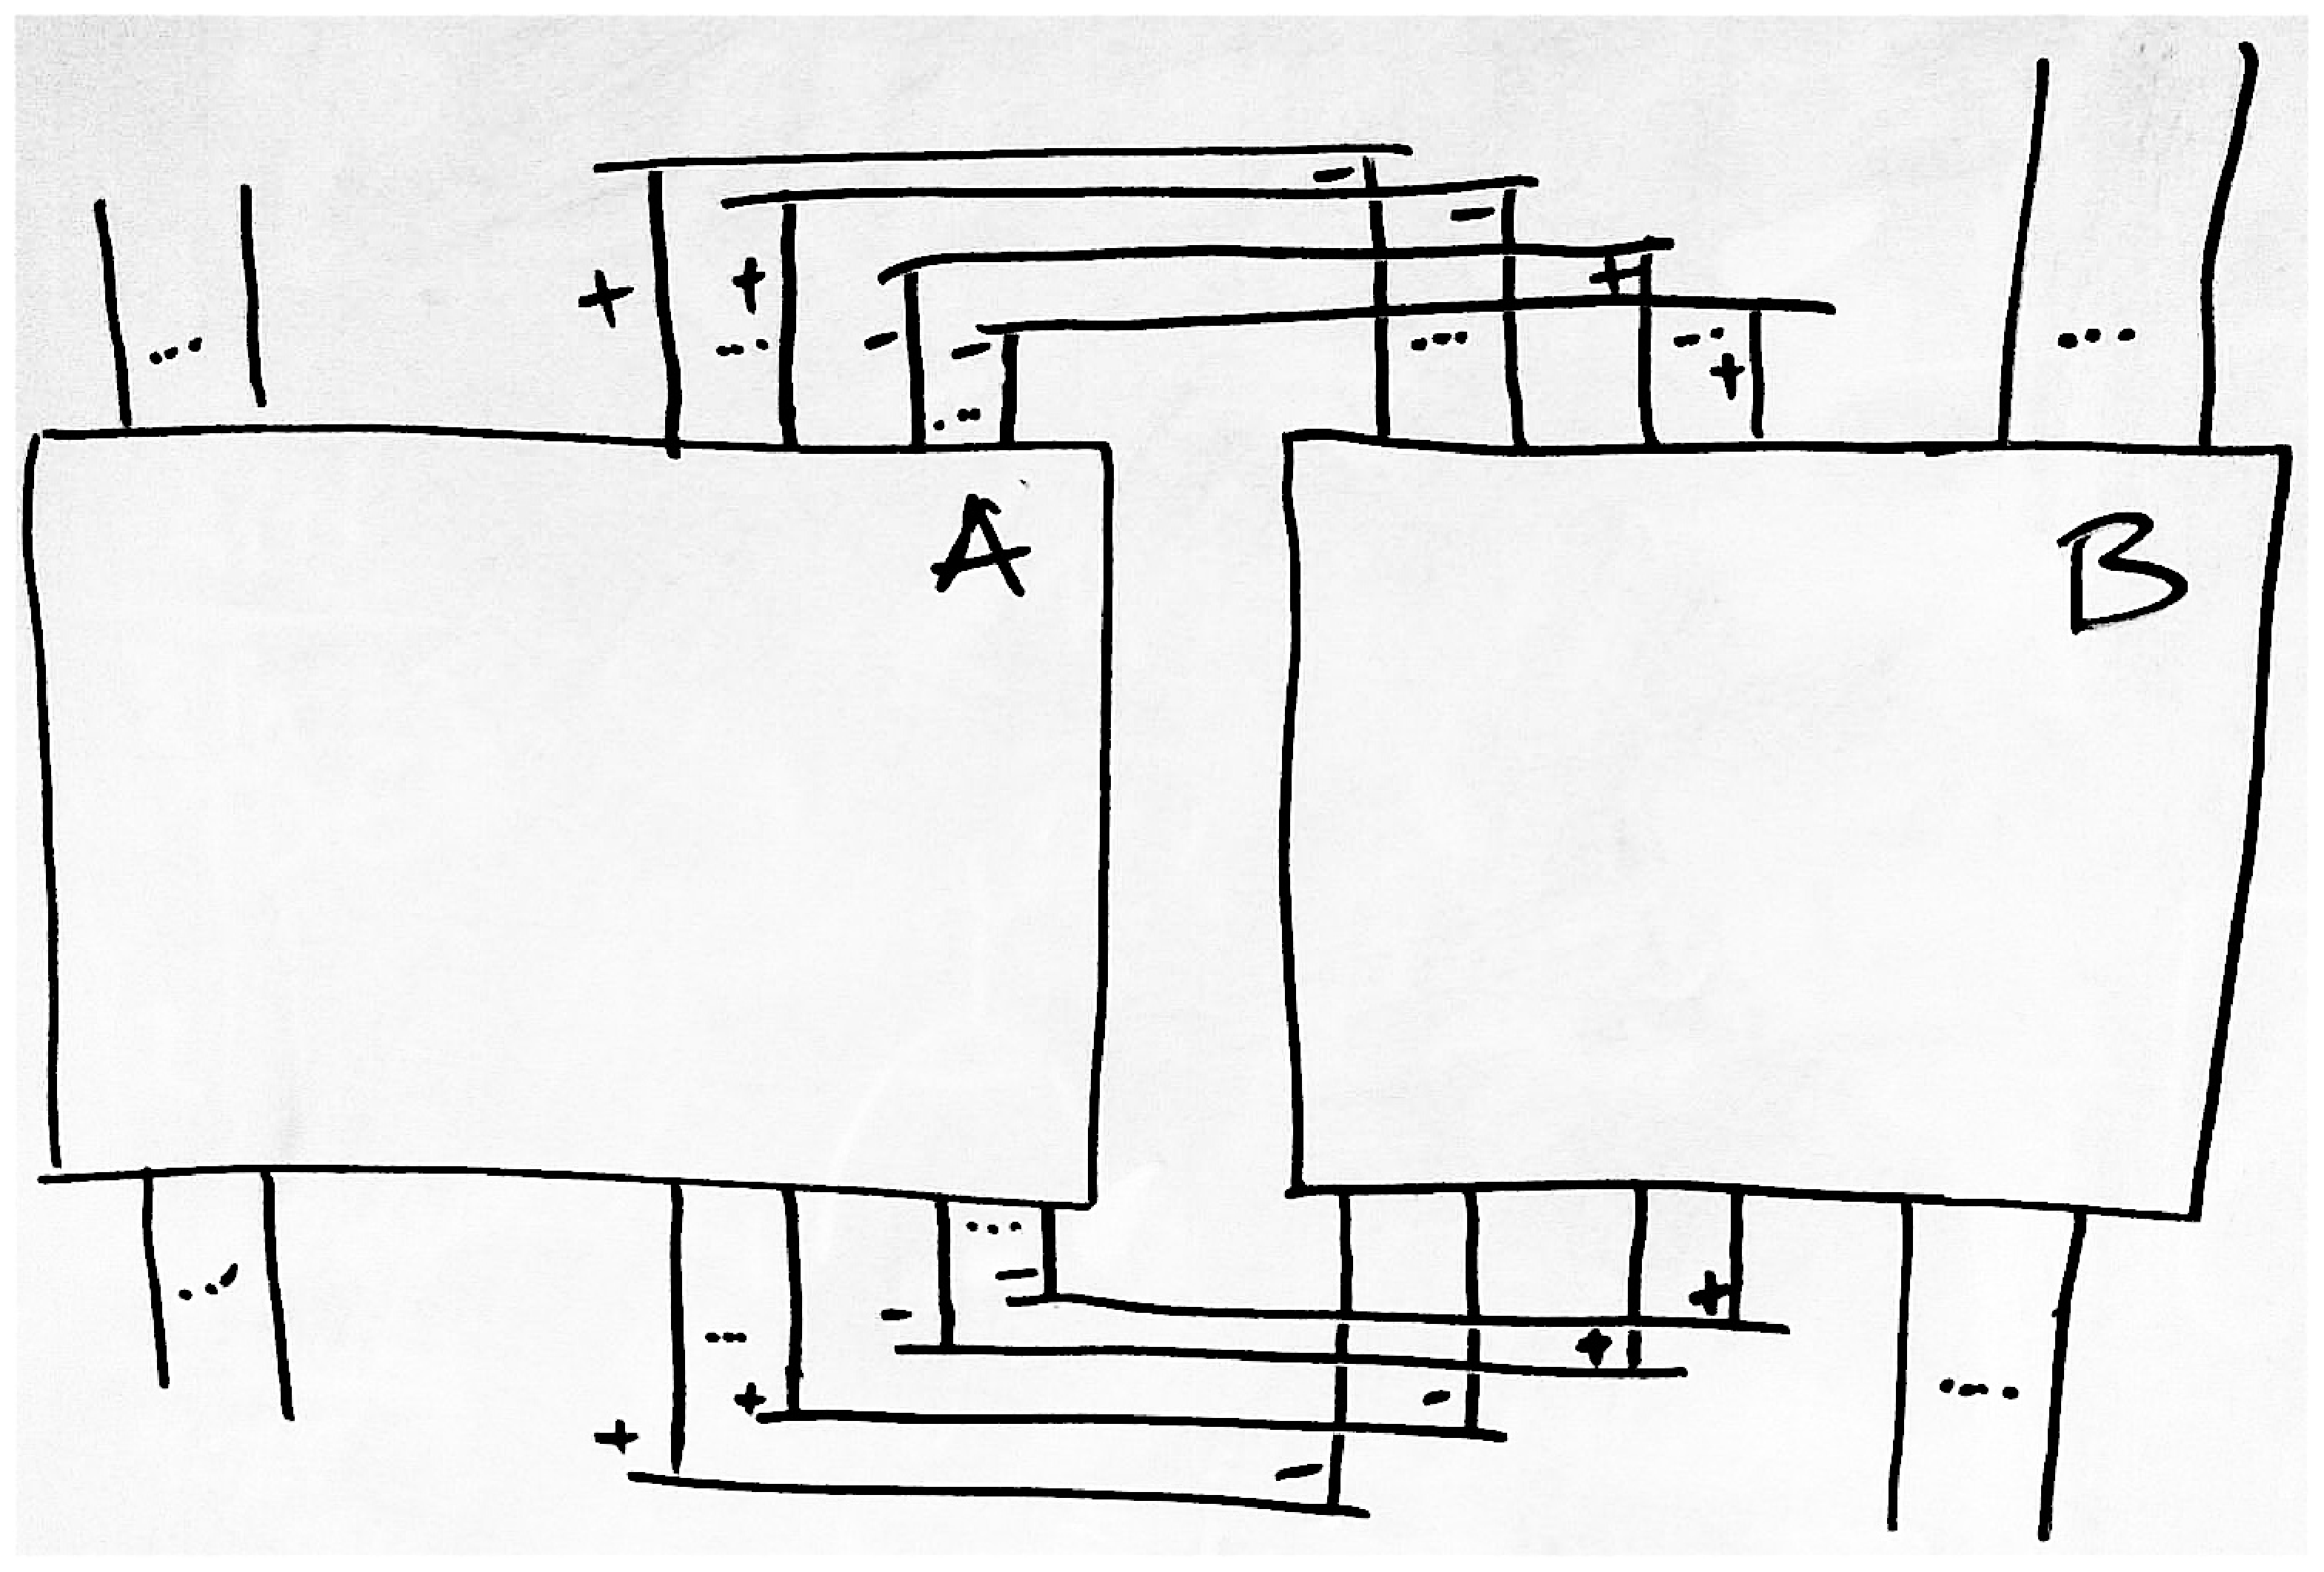
\includegraphics[width=2in]{original.eps} \\
                                &                           & $\downarrow$ \\
$\vlder{\Phi'}{}{\vls[\beta'.\delta]}{\vls(\alpha'.\gamma)}$ & $\rightarrow$ & $C'=$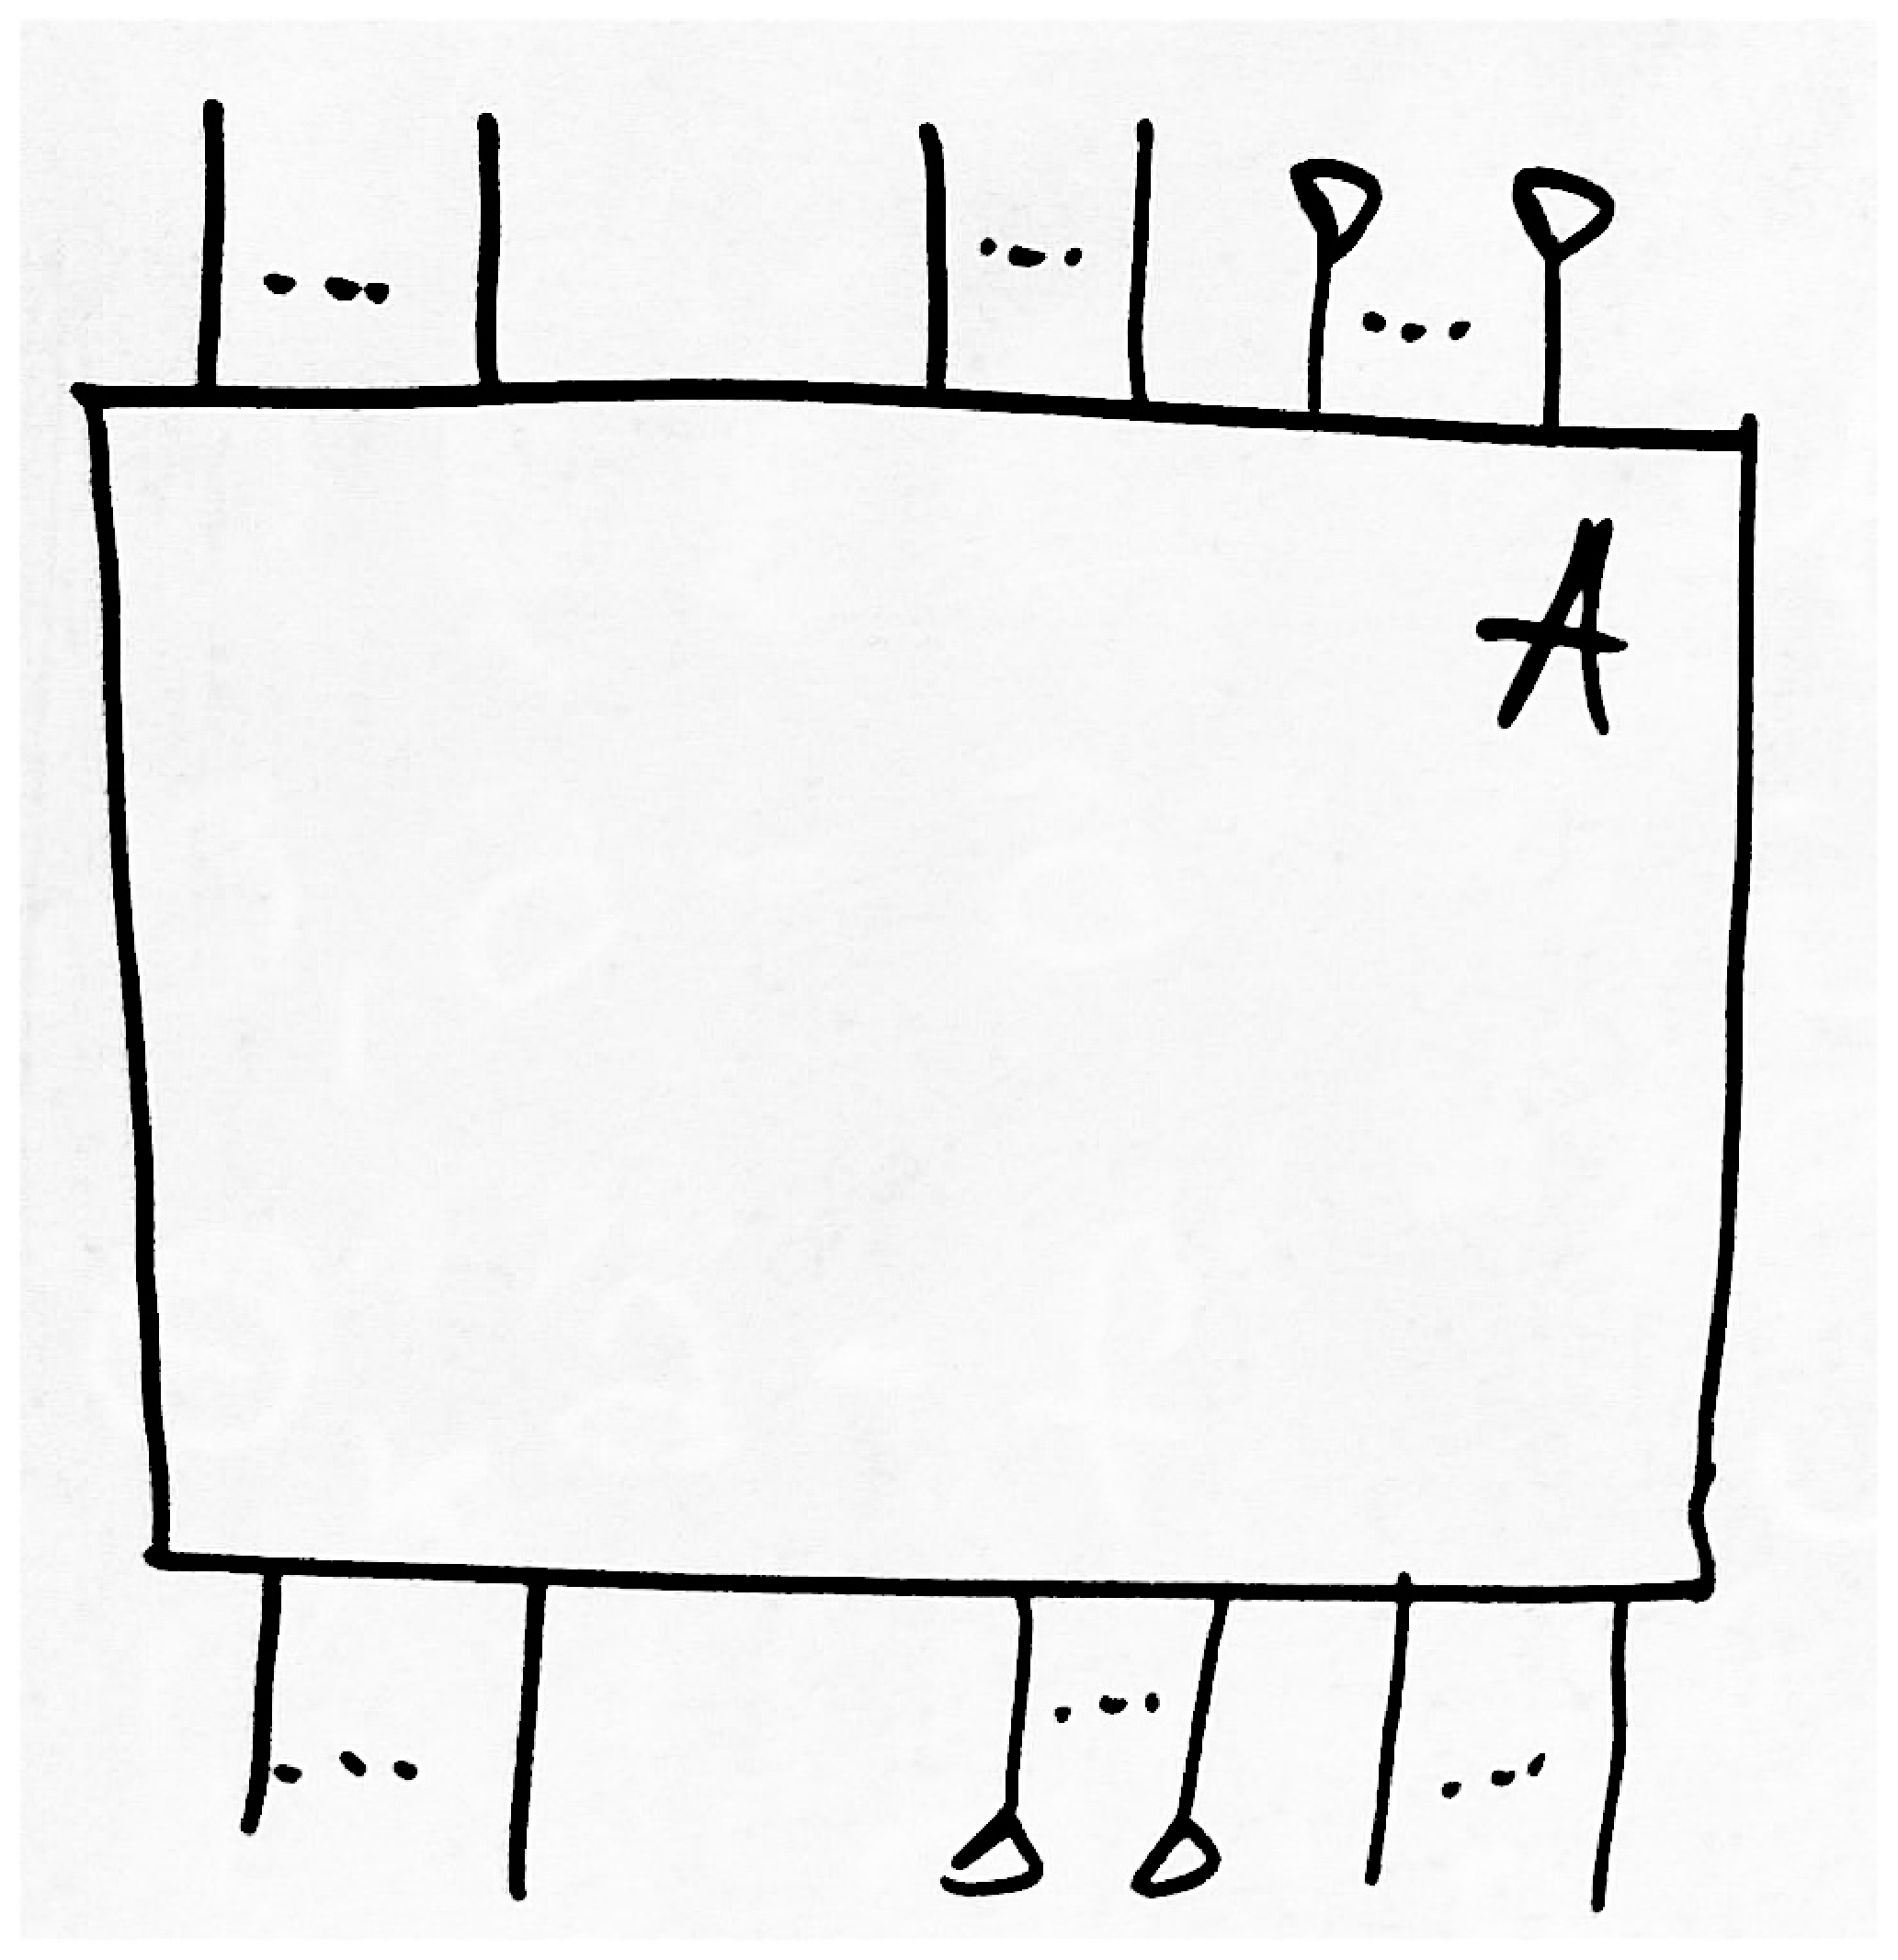
\includegraphics[width=1in]{experiment.eps}, \\
\end{tabular}
\newline
we say that
\begin{itemize}
\item $C'$ is an \emph{experiment on $C$ with respect to $B$ under $\pi$}; and
\item $\Phi'$ is an \emph{experiment on $\Phi$ with respect to $B$ under $\pi$} if
\begin{itemize}
 \item $\alpha'$ and $\beta'$ are obtained from $\alpha$ and $\beta$ respectively by substituting all the atoms mapping to positive (resp. negative) edges of $B$ with $\ttt$ (resp. $\fff$); and
 \item $\gamma$ (resp. $\delta$) is a conjuncton (resp. disjunction) of all the atoms mapping to top (resp. bottom) edges in $C'$, but not in $C$.
% TODO define ``top edge'' and ``bottom edge''
% \item $\gamma$ (resp. $\delta$) is a conjunction (resp. disjunction) of all the atoms mapping to edges adjacent to $\top$ (resp. $\bot$) in $C'$, but not in $C$.
\end{itemize}
\end{itemize}
\end{defi}

Given an atomic flow $C$ as described above, it is obvious that we can create the atomic flow $C'$. We now need to show that we can always obtain the corresponding derivation $\Phi'$, so in this sense making experiments is a ``sound'' operation.

\begin{lem}
Given any derivation $\Phi$ with atomic flow $C$, an atomic subflow $B$ of $C$ and a polarity assignment $\pi$, such that there exists an experiment on $C$ with respect to $B$ under $\pi$ then there exists a derivation $\Phi'$ such that $\Phi'$ is an experiment on $\Phi$ with respect to $B$ under $\pi$.
\end{lem}
\begin{proof}
Let $\Phi$ have premiss $\alpha$ and conclusion $\beta$, let $C'$ be an experiment on $C$ and let $\alpha'$, $\beta'$, $\xi'$ and $\zeta'$ denote the formulae obtained from $\alpha$, $\beta$, $\xi$ and $\zeta$ by substituting atoms mapping to positive (resp. negative) edges which occur in $C$ but not in $C'$ with $\ttt$ (resp. $\fff$). For simplicity, let us call the (co)interactions mapping to the (co)interaction nodes in $C$ which are not in neither $A$ nor $B$, \emph{evidenced (co)interactions}\footnote{we should consider to make this a proper definition, or if we want all the (co)interactions to be `evidenced'}.

We then obtain $\Phi'$ from $\Phi$ by substituting each formula $\xi$ with $\vls[(\xi'.\gamma_i).\delta_j]$; where $i$ (resp. $j$) is the number of evidenced interactions (resp. cointeractions) below (resp. above) $\xi$ in $\Phi$ such that the edge connecting the corresponding node to $A$ is positive (resp. negative) under $\pi$, $\gamma_0=\ttt$, $\gamma_{i}=\vls(\gamma_{i-1}.a_i)$, $\delta_0=\fff$ and $\delta_{j}=\vls[\delta_{j-1}.a_j]$; where $a_i$ (resp. $a_j$) is the atom, mapping to a positive edge, taking part in interaction (resp. cointeraction) number $i$ (resp. $j$) from the top (resp. bottom) in $\Phi$.

It is now straight forward to check that the following substitutions of inference rules gives a derivation with the right atomic flow:
\begin{itemize}
 \item Let $\vlinf{\rho}{}{\zeta}{\xi}$ be a linear inference rule or a structural inference rule mapping to a node in $A$, then it is substituted with $\vlinf{\rho}{}{\vls[(\zeta'.\gamma_i).\delta_j]}{\vls[(\xi'.\gamma_i).\delta_j]}$;
 \item let $\vlinf{\rho}{}{\zeta}{\xi}$ be a structural inference rule mapping to a node in $B$, then it is substituted with $\vlinf{=}{}{\vls[(\zeta'.\gamma_i).\delta_j]}{\vls[(\xi'.\gamma_i).\delta_j]}$\footnote{we might need a special case for $\vlinf{\rho}{}{\xi'\{\ttt\}}{\xi'\{\fff\}}$ where $\rho\in\{\awd,\awu\}$};
 \item let $\vlinf{\aid}{}{\xi\{\vls[a^\ppl.{\bar a}^\pmi]\}}{\xi\{\ttt\}}$ be an evidenced interaction rule, then if the edge connecting the node to $A$ is positive under $\pi$ it is substituted with $\vlinf{\sus}{}{\vls[(\xi'\{\vls[a^\ppl.\fff]\}.\gamma_i).\delta_j]}{\vls[(\xi'\{\ttt\}.\gamma_{i+1}).\delta_j]}$ otherwise it is substituted with $\vlinf{\awd}{}{\vls[(\xi'\{\vls[\ttt.{\bar a}^\pmi]\}.\gamma_i).\delta_j]}{\vls[(\xi'\{\ttt\}.\gamma_i).\delta_j]}$; and
 \item let $\vlinf{\aiu}{}{\xi\{\fff\}}{\xi\{\vls(a^\ppl.{\bar a}^\pmi)\}}$ be an evidenced cointeraction rule, then if the edge connecting the node to $A$ is negative under $\pi$ it is substituted with $\vlinf{\sus}{}{\vls[(\xi'\{\fff\}.\gamma_i).\delta_{j+1}]}{\vls[(\xi'\{\vls(\ttt.{\bar a}^\pmi)\}.\gamma_i).\delta_j]}$ otherwise it is substituted with $\vlinf{\awd}{}{\vls[(\xi'\{\vls[\ttt.{\bar a}^\pmi]\}.\gamma_i).\delta_j]}{\vls[(\xi'\{\ttt\}.\gamma_i).\delta_j]}$\footnote{note that there is no correspondence between negative and positive atoms and negative and positive polarities, the roles could be reversed. Alternatively we could do this without showing the atoms, but that might be too obfuscated?}.
\end{itemize}
The derivation $\Phi'$ we have obtained is a derivation from $\vls[(\alpha'.\gamma_k).\delta_0]$ to $\vls[(\beta'.\gamma_0).\delta_l]$ for some $k,l$, notice that $\gamma_0=\ttt$ and $\delta_0=\fff$, so we get $\Phi'$ from $\vls(\alpha'.\gamma_k)$ to $\vls[\beta'.\delta_l]$ as we want.
\end{proof}

When doing cut-elimination the experiments we need are of a specific form; we need to preserve the conclusion, so we cannot create any new bottom wires. This is the motivation for the following definition.

\begin{defi}
Let $C$ be an atomic flow and $\pi$ a polarity assignment to $C$. If $B$ is the subflow of $C$ containing only negative (resp. positive) nodes and $A$ is the subflow of $C$ containing only positive (resp. negative) nodes, then the experiment on $C$ with respect to $B$ under $\pi$ is called the \emph{$\fff$-experiment (resp. $\ttt$-experiment) on $C$ under $\pi$}. The definition extends to derivations in the obvious way.
\end{defi}

We now observe that a $\fff$-experiment indeed gives us the what we want. The observant reader might note that instead of the original conclusion, $\beta$, we get $\beta'$, which in this case is $\beta$ with some atom occurences substituted with $\fff$, as we shall se later, this is not a problem. We could indeed fix this straight away by applying $\awd$'s.

\begin{pro}\label{PropExperimentShapeBot}
For any proof\/ $\vlproof{\Pi}{\SKS}{\beta}$ and any polarity assignment to its atomic  flow, $\pi$, the $\fff$-experiment on $\Pi$ under $\pi$ is of the form $\vlder{}{\SKS\setminus\{\aid,\aiu\}}{\beta'}{\gamma}$. Where $\beta'$ and $\gamma$ are given by Definition~\ref{DefExperiment}.
\end{pro}

We have seen how we can generate one derivation for each polarity assignment, now we will see how we can glue all of these derivations together to get us the proof we want.

The disjunction of all the possible truth value assignments is obviously a tautology. We now show that we can construct a \emph{canonical} proof of this tautology. By ``canonical'' we mean that we can do it in such a way that there is no arbitrary choice involved. In particular this entails that the atomic flow of all the different atoms will be the same.

\begin{lem}\label{LemGlueTop}
Let $\Pi$ be a proof, let $\mathcal{P}$ be the set of all the polarity assignments to the atomic flow of $\Pi$ and for each $\pi\in\mathcal{P}$ let the $\fff$-experiment on $\Pi$ under $\pi$ have premiss $\gamma_\pi$. Then there exist \emph{canonical} proofs $\vlproof{}{\{\aid,\acu,\swi,\med\}}{\bigvee_{\pi\in\mathcal{P}}\gamma_\pi}$ and $\vlproof{}{\{\aid,\acd,\swi,\med\}}{\bigvee_{\pi\in\mathcal{P}}\gamma_\pi}$ of size $O(|\mathcal{P}|)$.
\end{lem}

\begin{proof}
Enumerate the atoms occurring in $\gamma_\pi$ for any $\pi$ $a_0,\dots,a_n$. Let $\pi_i$ be $\pi_{i+1}$ restricted to the subflow mapped to by $a_0,\dots,a_i$, let $\gamma_{\pi_i}=\gamma_\pi\{a_{i+1}\leftarrow\ttt,\dots,a_n\leftarrow\ttt\}$ and let $\mathcal{P}_i$ be the set of all the possible $\pi_i$. Notice that $|\mathcal{P}|=2^i$.

We induct on $i$. The inductive case becomes; $\vlproof{}{\{\aid,\acu,\swi,\med\}}{\bigvee_{\pi\in\mathcal{P_i}}\gamma_\pi}$

Given a subflow $A$ of the original atomic flow, let $\pi'$ be the restriction of $\pi$ to $A$. Then $\gamma_\pi'$ is obtained from $\gamma_\pi$ by substituting the atoms not in $\pi'$ with $\ttt$. Let $\gamma\in\mathcal{P}$ contain $n$ atoms, then define $\mathcal{P}_n=\mathcal{P}$ and $\mathcal{P}_{i-1}=\{\pi|\pi\in\mathcal{P}\}$
\end{proof}

\begin{lem}\label{LemGlueBottom}
Let $\Phi$ be a derivation from $\alpha$ to $\beta$, let $\mathcal{P}$ be the set of all the polarity assignments to the atomic flow of $\Phi$ and for each $\pi\in\mathcal{P}$ let the $\fff$-experiment on $\Phi$ under $\pi$ have conclusion $\beta_\pi$. Then there exists a derivation $\vlder{}{\{\acd,\med\}}{\beta}{\bigvee_{\pi\in\mathcal{P}}\beta_\pi}$.
\end{lem}

\begin{proof}
It is trivial to observe that there exists
\[
\vlderivation{
\vlde{}{\{\acd,\med\}}{\beta}
 {
  \vlde{}{\{\awd\}}{\bigvee_{\pi\in\mathcal{P}}\beta}
  {
   \vlhy{\bigvee_{\pi\in\mathcal{P}}\beta_\pi}
  }
 }
}
\]
Furthermore, observe that there is a path from every atom occurance in the conclusion to an atom occurence in the premise. Hence, all the $\awd$ rules are eliminate by applying weakening reductions to the derivaiton, giving us $\vlder{}{\{\acd,\med\}}{\beta}{\bigvee_{\pi\in\mathcal{P}}\beta_\pi}$ as required.
\end{proof}


\begin{thm}
Given a proof $\vlproof{\Pi}{\SKS}{\beta}$ there exists a canonical cut-free proof $\vlproof{}{\SKS\setminus\{\aiu\}}{\beta}$.
\end{thm}
\begin{proof}
Let $\mathcal{P}$ be the set of all the polarity assignments to the atomic flow of $\Pi$ and for each $\pi\in\mathcal{P}$ let the experiment on $\Pi$ under $\pi$ be $\vlder{\Pi_\pi}{\SKS\setminus\{\aid,\aiu\}}{\beta_\pi}{\gamma_\pi}$. Then by Lemma~\ref{LemGlueTop} and Lemma~\ref{LemGlueBottom} we can build the following proof:
\[
\vlderivation{
\vlde{}{\{\acd,\med\}}{\beta                                  } {
\vlde{\bigvee_{\pi\in\mathcal{P}}\Pi_\pi}
       {\SKS\setminus\{\aid,\aiu\}}{\bigvee_{\pi\in\mathcal{P}}\beta_\pi}{
\vlpr{}{\{\aid,\acu,\swi\}}{\bigvee_{\pi\in\mathcal{P}}\gamma_\pi       }}}
}\quad.
\]
There is only one way of building such a proof in the sense that the atomic flow of the proof will be unique (modulo associativity of contraction).
\end{proof}

%%===============================================================================
%\section{Interpolation}

%\begin{defi}\label{DefExperiment2}
%Let $\vlder{\Psi}{\{\aid,\aiu,\swi,\med\}}{\beta}{\alpha}$ be a streamlined derivation, then we call $\vlder{\Psi_p}{\{\aid,\aiu,\swi,\med\}}{\beta_p}{\alpha_p}$ an \emph{experiment on $\Psi$ under polarity assignment $\pi_p$ with respect to atomic flow $A$} if $\Psi_p$ is obtained from $\Psi$ by
%\begin{itemize}
%\item replacing each $\vlinf{\aid}{}{\xi\{\vls[a_i^\ppl.{\bar a_i^\pmi}]\}}{\xi\{\ttt\}}$ mapping to a node in $A$ by $\vlinf{=}{}{\xi_p\vlsbr[\ttt.\fff]}{\xi_p\{\ttt\}}$, for some $0 \leq i \leq n$;
%\item replacing each $\vlinf{\aiu}{}{\xi\{\fff\}}{\xi\{\vls(a_i^\ppl.{\bar a_i^\pmi})\}}$ mapping to a node in $A$ by $\vlinf{=}{}{\xi_p\{\fff\}}{\xi_p\vlsbr(\ttt.\fff)}$, for some $0 \leq i \leq n$; and
%\item replacing each other rule instance $\vlinf{\rho}{}{\xi}{\zeta}$ by $\vlinf{\rho}{}{\xi_p}{\zeta_p}$,
%\end{itemize}
%where $\rho\in\{\swi,\med\}$ and $\alpha_p,\beta_p,\xi_p,\zeta_p$ denote the formulae obtained from $\alpha,\beta,\xi,\zeta$, respectively, by replacing atom occurrences mapped to edges of $A$. Atoms mapping to positive (resp. negative) edges under $\pi_p$ are replaced with $\ttt$ (resp. $\fff$).
%\end{defi}

%\begin{rem}
%If we define a $\top$-experiment to be the dual of a $\bot$-experiment in the usual way, then an \emph{experiment} on $\Psi$ is exactly a $\top$-experiment on a $\bot$-experiment on $\Psi$ (or the other way around) (under the same polarity assignment, with respect to the same atomic flow).
%\end{rem}

%\begin{pro}
%If $\Psi_p$ is an experiment on $\Psi$ with respect to the atomic flow containing all the $\aid$ nodes of $\Psi$, then $\Psi_p$ is a valid derivation.
%\end{pro}

%\begin{pro}\label{PropExperimentShape}
%An experiment under polarity assignment $\pi_p$ on a streamlined derivation\/ $\vlder{\Psi}{\{\aid,\aiu,\swi,\med\}}{\beta}{\alpha}$ with respect to an atomic flow containing all the $\aid$ nodes of $\Psi$ is of the form $\vlder{}{\{\aiu,\swi,\med\}}{\beta_p}{\alpha}$. Where $\beta_p$ is given by Definition~\ref{DefExperiment2}.
%\end{pro}

%\begin{lem}\label{LemGlue}
%Given a derivation $\vlder{\Psi}{}{\beta}{\alpha}\ $, and all the experiments on $\Pi$ with respect to a given atomic flow there exists a derivation $\vlder{}{\{\aid,\swi\}}{\bigvee_{p=1}^{2^n}\beta_p^\bot}{\bigwedge_{p=1}^{2^n}\beta_p}$, where $\beta^\bot_p$ is given by Definition~\ref{DefExperiment}.
%\end{lem}

%\begin{lem}\label{LemInterpolant}
%Given a streamlined derivation of the form
%\[
%\vlder{\Psi}{\{\aid,\aiu,\swi,\med\}}{\beta}{\alpha}
%\]
%there is a derivation, $\Psi'$, of the form
%\[
%\vlderivation{
%\vlde{}{\{\aid,\acd,\swi,\med\}}{\beta} {
%\vlde{}{\{\aiu,\acu,\swi,\med\}}{\gamma}{
%\vlhy{\alpha}}}
%}
%\]
%\end{lem}

%\begin{proof}
%Consider all the experiments on $\Psi$; $\Psi_1,\dots,\Psi_{2^n}$. Using these derivations and Lemma~\ref{LemGlueBottom} and Lemma~\ref{LemGlue} we can build:
%\[
%\vlderivation{
%\vlde{}{\{\acd,\med\}}     {\beta                          }   {
%\vlde{}{\{\aid,\swi\}}     {\bigvee_{p=1}^{2^n}\beta^\bot_p}  {
%\vlde{\bigwedge_{p=1}^{2^n}\Psi_p}{\{\aiu,\swi,\med\}}
%                           {\bigwedge_{p=1}^{2^n}\beta_p   } {
%\vlde{}{\{\acu,\med\}}     {\bigwedge_{p=1}^{2^n}\alpha    }{
%\vlhy                      {\alpha                         }}}}}
%}\quad,
%\]
%Where $\gamma=\bigwedge_{p=1}^{2^n}\beta_p$.
%\end{proof}

%\begin{pro}
%If there exists a derivation like $\Psi'$ in Lemma~\ref{LemInterpolant}, then $\gamma$ is an interpolant of $\alpha$ and $\beta$.
%\end{pro}

%===============================================================================
\section{Streamlining}

We want to show two things in this section. Firstly that any subflow with no path to either $\top$ nor $\bot$ can be eliminated (at the expense of copying the rest of the flow). Secondly that we can transform an atomic flow in such a way that every path from an interaction to a cointeraction node is in a subflow which is not connected to $\top$ nor $\bot$. We do the latter first.

\begin{defi}
We call an atomic flow \emph{ambiguous} for polarity assignment $\pi_p$ if there exist an interaction (resp. cointeraction) node with a positive path from the interaction (resp. cointeraction) to $\bot$ (resp. $\top$) and a positive path from the interaction (resp. cointeraction) node to a cointeraction (resp. interaction node). If an atomic flow is not ambiguous for plority assignment $\pi_p$ we say that it is \emph{unambiguous}.
\end{defi}

\begin{lem}
Given a derivation $\Delta$ from $\alpha$ to $\beta$ with atomic flow $A$ there exists a derivation $\Delta'$ from $\alpha$ to $\beta$ with unambiguous atomic flow $A'$ for some polarity assignment $\pi_p$ such that $|A'|/|A|\in O(1)$.
\end{lem}

\begin{proof}[Proof (Sketch)]
{\footnotesize\begin{verbatim}
Here is the picture. In constructions 1-3, a,b,c,d (which are just labels, and
not atom names) are supposed to represent groups of wires (but I have drawn only
one for simplicity).

1) The construction Alessio found when there is one group of top wires, and two
groups of bottom wires. In the derivation this is obtained by substituting "a
\leftarrow a \land a".

2) The dual of 1.

3) Consider group a and b as one group and apply (1). Now consider c and d as
one group and apply (2). Finally apply some weakening reductions. The result is
four boxes, one with paths from a to c, one with path from a to d, one with
paths from b to c and one with paths from a to d.

4) (3) applied to the case we are interested in, where a go to interactions and
c to cuts. I labelled the four boxes, to show that I shuffled them around a bit
for readability. Box 1 is eliminated and 2-4 kept.
\end{verbatim}}

\[
\atomicflow{
(-2,8)*{\afvj4};
(0,8)*{\cdots};
(2,8)*{\afvj4};
(0,0)*{\affr{12}{12}};
(-5,-8)*{\afvj4};
(-3,-8)*{\cdots};
(-1,-8)*{\afvj4};
(5,-8)*{\afvj4};
(3,-8)*{\cdots};
(1,-8)*{\afvj4};
}\quad\rightarrow\quad
\atomicflow{
(-2,12)*{\afacuexsq{}{}{}{}{}{}{4}{1}};
(0,16)*{\cdots};
(2,12)*{\afacuexsq{}{}{}{}{}{}{4}{1}};
(-8,0)*{\affr{12}{12}};
(8,0)*{\affr{12}{12}};
(-13,-8)*{\afvj4};
(-11,-8)*{\cdots};
(-9,-8)*{\afvj4};
(-3,-10)*{\afawu{}{}{}{}};
(-5,-8)*{\cdots};
(-7,-10)*{\afawu{}{}{}{}};
(13,-8)*{\afvj4};
(11,-8)*{\cdots};
(9,-8)*{\afvj4};
(3,-10)*{\afawu{}{}{}{}};
(5,-8)*{\cdots};
(7,-10)*{\afawu{}{}{}{}};
}
\]

\[
\atomicflowinv{
(-2,8)*{\afvj4};
(0,8)*{\cdots};
(2,8)*{\afvj4};
(0,0)*{\affr{12}{12}};
(-5,-8)*{\afvj4};
(-3,-8)*{\cdots};
(-1,-8)*{\afvj4};
(5,-8)*{\afvj4};
(3,-8)*{\cdots};
(1,-8)*{\afvj4};
}\quad\rightarrow\quad
\atomicflow{
(-2,-12)*{\afacdexsq{}{}{}{}{}{}{4}{1}};
(0,-16)*{\cdots};
(2,-12)*{\afacdexsq{}{}{}{}{}{}{4}{1}};
(-8,0)*{\affr{12}{12}};
(8,0)*{\affr{12}{12}};
(-13,8)*{\afvj4};
(-11,8)*{\cdots};
(-9,8)*{\afvj4};
(-3,10)*{\afawd{}{}{}{}};
(-5,8)*{\cdots};
(-7,10)*{\afawd{}{}{}{}};
(13,8)*{\afvj4};
(11,8)*{\cdots};
(9,8)*{\afvj4};
(3,10)*{\afawd{}{}{}{}};
(5,8)*{\cdots};
(7,10)*{\afawd{}{}{}{}};
}
\]

\[
\atomicflowinv{
(-5,8)*{\afvj4};
(-3,8)*{\cdots};
(-1,8)*{\afvj4};
(5,8)*{\afvj4};
(3,8)*{\cdots};
(1,8)*{\afvj4};
(0,0)*{\affr{12}{12}};
(-5,-8)*{\afvj4};
(-3,-8)*{\cdots};
(-1,-8)*{\afvj4};
(5,-8)*{\afvj4};
(3,-8)*{\cdots};
(1,-8)*{\afvj4};
}\quad\rightarrow\quad
\atomicflow{
(-21,16)*{\afacuexsq{}{}{}{}{}{}{4}{1}};
(-19,20)*{\cdots};
(-17,16)*{\afacuexsq{}{}{}{}{}{}{4}{1}};
%---
(21,16)*{\afacuexsq{}{}{}{}{}{}{4}{1}};
(19,20)*{\cdots};
(17,16)*{\afacuexsq{}{}{}{}{}{}{4}{1}};
%---
(-25,8)*{\afvj4};
(-29,8)*{\afvj4};
%---
(-19,10)*{\afawd{}{}{}{}};
(-21,8)*{\cdots};
(-23,10)*{\afawd{}{}{}{}};
%---
(-9,8)*{\afvj4};
(-13,8)*{\afvj4};
%---
(-3,10)*{\afawd{}{}{}{}};
(-5,8)*{\cdots};
(-7,10)*{\afawd{}{}{}{}};
%---
(3,10)*{\afawd{}{}{}{}};
(5,8)*{\cdots};
(7,10)*{\afawd{}{}{}{}};
%---
(9,8)*{\afvj4};
(13,8)*{\afvj4};
%---
(19,10)*{\afawd{}{}{}{}};
(21,8)*{\cdots};
(23,10)*{\afawd{}{}{}{}};
%---
(25,8)*{\afvj4};
(29,8)*{\afvj4};
%---
(-24,0)*{\affr{12}{12}};
(-8,0)*{\affr{12}{12}};
(8,0)*{\affr{12}{12}};
(24,0)*{\affr{12}{12}};
%---
(-25,-8)*{\afvj4};
(-29,-8)*{\afvj4};
%---
(-19,-10)*{\afawu{}{}{}{}};
(-21,-8)*{\cdots};
(-23,-10)*{\afawu{}{}{}{}};
%---
(-9,-10)*{\afawu{}{}{}{}};
(-11,-8)*{\cdots};
(-13,-10)*{\afawu{}{}{}{}};
%---
(-3,-8)*{\afvj4};
(-7,-8)*{\afvj4};
%---
(3,-8)*{\afvj4};
(7,-8)*{\afvj4};
%---
(9,-10)*{\afawu{}{}{}{}};
(11,-8)*{\cdots};
(13,-10)*{\afawu{}{}{}{}};
%---
(19,-10)*{\afawu{}{}{}{}};
(21,-8)*{\cdots};
(23,-10)*{\afawu{}{}{}{}};
%---
(25,-8)*{\afvj4};
(29,-8)*{\afvj4};
%---
(-13,-16)*{\afacdexsq{}{}{}{}{}{}{8}{1}};
(-11,-20)*{\cdots};
(-9,-16)*{\afacdexsq{}{}{}{}{}{}{8}{1}};
%---
(13,-16)*{\afacdexsq{}{}{}{}{}{}{8}{1}};
(11,-20)*{\cdots};
(9,-16)*{\afacdexsq{}{}{}{}{}{}{8}{1}};
}
\]
\end{proof}

\begin{defi}\label{DefRedIS}
We define the reduction $\rightarrow_{is}$ (where $is$ stands for \emph{isolated subflow}) as follows, for all atomic flows $A$ and $B$:

where $h,k\geq0$, edges have been renamed with accents, flows $\tilde{A}$ and $\hat{A}$ are both isomorphic to $A$ and $B$ is connected.
\end{defi}

\begin{thm}
Reduction $\rightarrow_{is}$ is sound.
\end{thm}
\begin{proof}
Let $\Phi$ be a derivation with flow $C$, such that $C\rightarrow_{si} D$. We show that there exists a derivation $\Psi$ with flow $D$ and with the same premiss and conclusion as $\Phi$. In the following we refer to the figure in Definition~\ref{DefRedIS}. We assume that $\Phi$ has premiss $\xi$ and conclusion $\zeta$. Now we will conduct experiments with respect to $B$. Since $B$ is connected we know that it has two polarity assignments $\pi_+$ and $\pi_-$, where each polarity assignment assigns the given polarity to all the edges in $B$. Now let $\Phi_+^\top$ be the $\top$-experiment under $\pi_+$ and let $\Phi_-^\bot$ be the $\bot$-experiment under $\pi_-$ both with respect to $B$. Then we have:
\[
\vlder{\Phi_+^\top}{}{\vls[\zeta.{\bar a}.\cdots.{\bar a}]}{\xi}
,\quad
\vlder{\Phi_-^\bot}{}{\zeta}{\vls({\bar a}.\cdots.{\bar a}.\xi)}
\]
We can now connect the two experiments to get the desired derivation:
\[
\vlderivation{
\vlin{\cod}{}{\zeta}{
\vlde{\vls[\zeta.\Phi_+^\top]}{}{\vls[\zeta.\zeta]}{
\vlin{\acu^\star}{}{\vls[\zeta.({\bar a}.\cdots.{\bar a}.\xi)]}{
\vlin{\swi}{}{\vls[\zeta.({\bar a}.\xi)]}{
\vlin{\acd^\star}{}{\vls([\zeta.{\bar a}].\xi)}{
\vlde{\vls(\Phi_-^\bot.\xi)}{}{\vls([\zeta.{\bar a}.\cdots.{\bar a}].\xi)}{
\vlin{\cou}{}{\vls(\xi.\xi)}{
\vlhy{\xi}}}}}}}}
}
\]
\end{proof}

\iflmcs\else\let\oldurl\url\renewcommand{\url}[1]{\hfill\break\oldurl{#1}}\fi

\bibliographystyle{alpha}
\bibliography{di-biblio}

\end{document}